\chapter{Affichage du résultat}
	Après avoir réaliser la fonction de calcul du résultat il convient d'en réaliser sa fonction d'affichage. 
    Nous avons trouvé que la méthode d'affichage en binaire proposée dans le cadre du projet n'était pas forcément des plus intuitive à comprendre.
    
    En conséquence nous en avons cherché une nouvelle plus facile à comprendre pour un néophyte.
    
\section{L'affichage retenu}
	Comme nous sommes sur un afficheur où chaque caractères est constitué de 5x8 pixels, nous avons choisi l'affichage que vous pouvez voir sur la figure \ref{affichagefull} avec sur la gauche autant de lignes que d'éléments bien placés et à droite autant de lignes que de bons éléments mais mal placés
    
  Pour davantage de facilités à lire et à implémenter également, nous avons disposés les lignes alternativement.
  
    \begin{figure}[h]
        \centering
        \subfloat[Affichage de toutes les possibilités]{\label{affichagefull}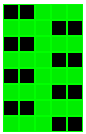
\includegraphics[width=3cm]{affichageResultatFull.png}}    
        \hspace{5pt}
        \subfloat[Dans le cas où on en a 3 bien placés et 1 mal placé]{\label{affichage32}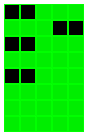
\includegraphics[width=3cm]{affichageResultat31.png}}
        \hspace{5pt}
        \subfloat[Dans le cas où on en a 0 de bien placés et 2 de mal placé]{\label{affichage02}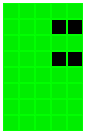
\includegraphics[width=3cm]{affichageResultat02.png}}
        
        \subfloat[En situation de jeu dans le cas ou la réponse secrète est DBAE]{\label{affichageEx}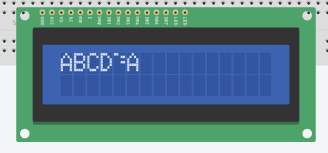
\includegraphics[height=4cm]{affichageResultEx.png}}
        \caption{Exemples de résultats obtenus}
        \label{affichages}
    \end{figure}

  
\section{Le programme}
	Pour parvenir au résultat ci-dessus nous avons utilisé la fonction \og createChar()\footnotemark \fg de la librairie LiquidCrystal.
	Pour faire un bref résumé, c'est une fonction qui permet de créer un caractère pixel par pixel.
    A cette fin il y a 8 caractères de la librairie qui sont disponible (de 0 à 8).
    Ceci est possible car dans la libraire LiquidCrystal les caractères sont sous la forme suivante:
  
  \begin{lstlisting}
byte smiley[8] = {
    B00000,
    B10001,
    B00000,
    B00000,
    B10001,
    B01110,
    B00000,
};
  \end{lstlisting}
  
  
  C'est un tableau de type byte ou chaque \og B***** \fg (byte) définit une ligne, chaque \og * \fg peut valoir 0 ou 1. 
  On peut donc éteindre ou allumer chaque pixels de chaque lignes indépendamment.
  
\paragraph{}
\underline{Programme d'affichage des résultats:}
\lstinputlisting{Sources/TestAffichage.ino}
    
\footnotetext {voir la page:\href{https://www.arduino.cc/en/Reference/LiquidCrystalCreateChar}{arduino.cc}}  